\documentclass[13pt,onlymath]{beamer}
\usefonttheme{serif}
\usepackage{graphicx,amsmath,amssymb,tikz,psfrag,epstopdf,fancyvrb}
\usepackage[lighttt]{lmodern}
%\usepackage{graphicx,psfrag}

\input defs.tex

%% formatting

\mode<presentation>
{
\usetheme{default}
}
\setbeamertemplate{navigation symbols}{}
\usecolortheme[rgb={0.13,0.28,0.59}]{structure}
\setbeamertemplate{itemize subitem}{--}
\setbeamertemplate{frametitle} {
    \begin{center}
      {\large\bf \insertframetitle}
    \end{center}
}

\newcommand\footlineon{
  \setbeamertemplate{footline} {
    \begin{beamercolorbox}[ht=2.5ex,dp=1.125ex,leftskip=.8cm,rightskip=.6cm]{structure}
      \footnotesize \insertsection
      \hfill
      {\insertframenumber}
    \end{beamercolorbox}
    \vskip 0.45cm
  }
}
\footlineon

\AtBeginSection[] 
{ 
    \begin{frame}<beamer> 
        \frametitle{Outline} 
        \tableofcontents[currentsection,currentsubsection] 
    \end{frame} 
} 

%% begin presentation

\title{\large \bfseries Dynamic Programming}

\author{Jaehyun Park\\[3ex]
CS 97SI\\
Stanford University}

\date{\today}

\begin{document}

\frame{
\thispagestyle{empty}
\titlepage
}

\section{Dynamic Programming}

\begin{frame}{What is DP?}
\BIT
\item Wikipedia definition: ``method for solving complex problems by breaking them down into simpler subproblems''
\vfill
\item This definition will make sense once we see some examples
\BIT
\item Actually, we'll only see problem solving examples today
\EIT
\EIT
\end{frame}

\begin{frame}{Steps for Solving DP Problems}
\begin{enumerate}
\item Define subproblems
\item Write down the recurrence that relates subproblems
\item Recognize and solve the base cases
\end{enumerate}
\vfill
\BIT
\item Each step is very important!
\EIT
\end{frame}

\section{1-dimensional DP}

\begin{frame}{1-dimensional DP Example}
\BIT
\item Problem: given $n$, find the number of different ways to write $n$ as the sum of 1, 3, 4
\item Example: for $n=5$, the answer is 6
\BEAS
5 &=& 1+1+1+1+1 \\ &=& 1+1+3 \\ &=& 1+3+1 \\ &=& 3+1+1 \\ &=& 1+4 \\ &=& 4+1
\EEAS
\EIT
\end{frame}

\begin{frame}{1-dimensional DP Example}
\BIT
\item Define subproblems
\BIT
\item Let $D_n$ be the number of ways to write $n$ as the sum of 1, 3, 4
\EIT
\item Find the recurrence
\BIT
\item Consider one possible solution $n = x_1 + x_2 + \cdots + x_m$
\item If $x_m = 1$, the rest of the terms must sum to $n-1$
\item Thus, the number of sums that end with $x_m=1$ is equal to $D_{n-1}$
\item Take other cases into account ($x_m=3$, $x_m=4$)
\EIT
\EIT
\end{frame}

\begin{frame}{1-dimensional DP Example}
\BIT
\item Recurrence is then
\[
D_n = D_{n-1} + D_{n-3} + D_{n-4}
\]
\item Solve the base cases
\BIT
\item $D_0 = 1$
\item $D_n = 0$ for all negative $n$
\item Alternatively, can set: $D_0 = D_1 = D_2 = 1$, and $D_3 = 2$
\EIT
\vfill
\item We're basically done!
\EIT
\end{frame}

\begin{frame}[fragile]{Implementation}
\begin{Verbatim}[xleftmargin=25pt]
D[0] = D[1] = D[2] = 1; D[3] = 2;
for(i = 4; i <= n; i++)
    D[i] = D[i-1] + D[i-3] + D[i-4];
\end{Verbatim}
\BIT
\item Very short!
\item Extension: solving this for huge $n$, say $n \approx 10^{12}$
\BIT
\item Recall the matrix form of Fibonacci numbers
\EIT
\EIT
\end{frame}

\begin{frame}{POJ 2663: Tri Tiling}
\BIT
\item Given $n$, find the number of ways to fill a $3 \times n$ board with dominoes
\vfill
\item Here is one possible solution for $n=12$
\begin{center}
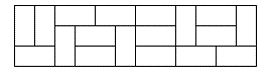
\includegraphics[height=0.3\textheight]{figures/tritiling}
\end{center}
\EIT
\end{frame}

\begin{frame}{POJ 2663: Tri Tiling}
\BIT
\item Define subproblems
\BIT
\item Define $D_n$ as the number of ways to tile a $3 \times n$ board
\EIT
\vfill
\item Find recurrence
\BIT
\item Uuuhhhhh...
\EIT
\EIT
\end{frame}

\begin{frame}{Troll Tiling}
\begin{center}
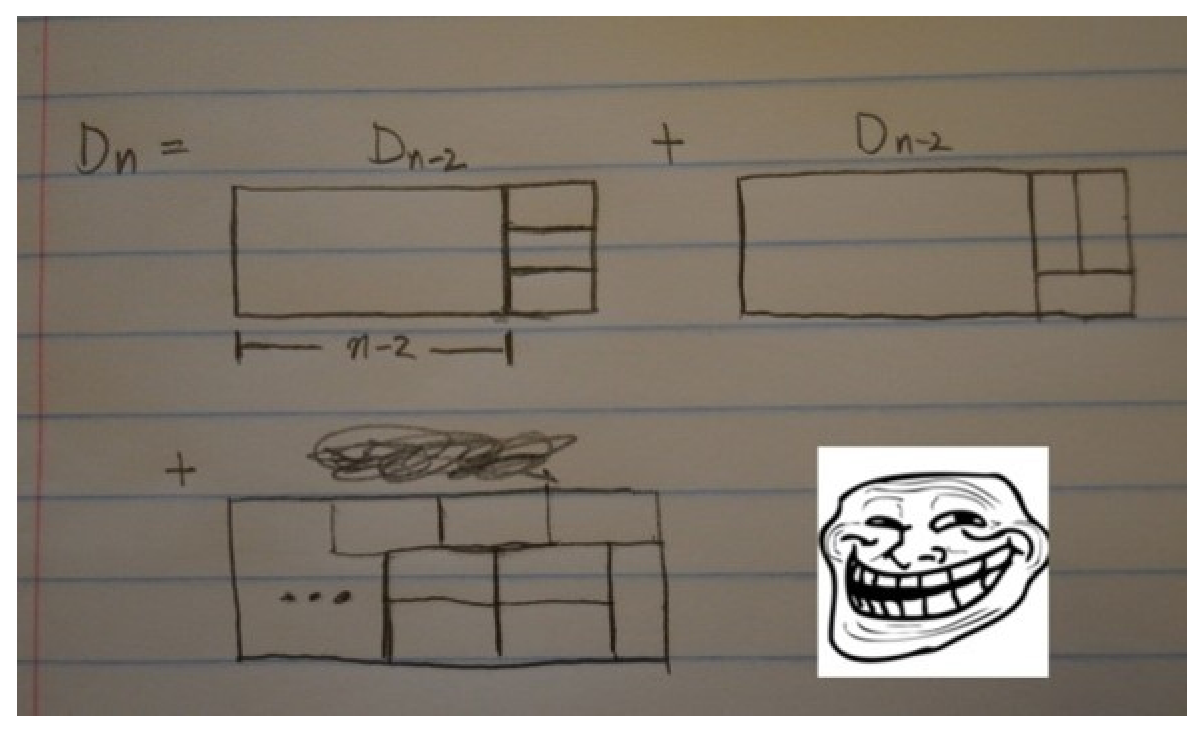
\includegraphics[height=0.7\textheight]{figures/trolltiling}
\end{center}
\end{frame}

\begin{frame}{Defining Subproblems}
\BIT
\item Obviously, the previous definition didn't work very well
\item $D_n$'s don't relate in simple terms
\vfill
\item What if we introduce more subproblems?
\EIT
\end{frame}

\begin{frame}{Defining Subproblems}
\begin{center}
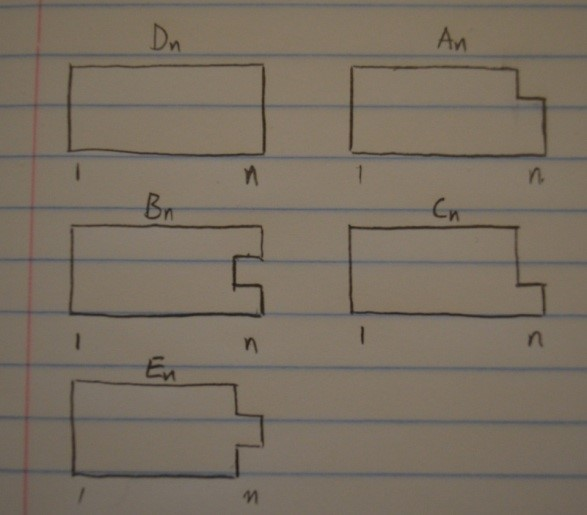
\includegraphics[height=0.7\textheight]{figures/tritiling_sub1}
\end{center}
\end{frame}

\begin{frame}{Finding Recurrences}
\begin{center}
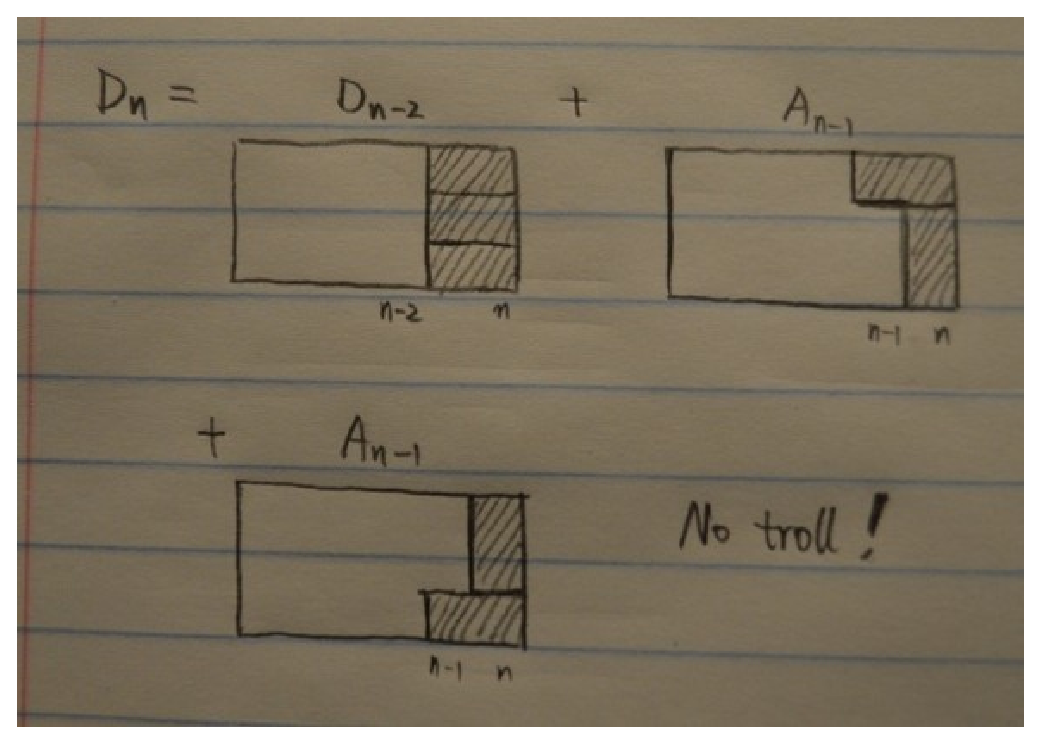
\includegraphics[height=0.7\textheight]{figures/tritiling_sub2}
\end{center}
\end{frame}

\begin{frame}{Finding Recurrences}
\BIT
\item Consider different ways to fill the $n$th column
\BIT \item And see what the remaining shape is \EIT
\item Exercise:
\BIT
\item Finding recurrences for $A_n$, $B_n$, $C_n$
\item Just for fun, why is $B_n$ and $E_n$ always zero?
\EIT
\vfill
\item Extension: solving the problem for $n \times m$ grids, where $n$ is small, say $n \le 10$
\BIT \item How many subproblems should we consider? \EIT
\EIT
\end{frame}

\section{2-dimensional DP}

\begin{frame}[fragile]{2-dimensional DP Example}
\BIT
\item Problem: given two strings $x$ and $y$, find the longest common subsequence (LCS) and print its length
\item Example:
\BIT
\item $x$: {\ttfamily A{\bfseries BC}BD{\bfseries AB}}
\item $y$: {\ttfamily {\bfseries B}D{\bfseries CAB}C}
\item ``\texttt{BCAB}'' is the longest subsequence found in both sequences, so the answer is 4
\EIT
\EIT
\end{frame}

\begin{frame}{Solving the LCS Problem}
\BIT
\item Define subproblems
\BIT
\item Let $D_{ij}$ be the length of the LCS of $x_{1\ldots i}$ and $y_{1\ldots j}$
\EIT
\item Find the recurrence
\BIT
\item If $x_i = y_j$, they both contribute to the LCS
\BIT
\item $D_{ij} = D_{i-1, j-1} + 1$
\EIT
\item Otherwise, either $x_i$ or $y_j$ does not contribute to the LCS, so one can be dropped
\BIT
\item $D_{ij} = \max\{D_{i-1,j}, D_{i, j-1}\}$
\EIT
\item Find and solve the base cases: $D_{i0} = D_{0j} = 0$
\EIT
\EIT
\end{frame}

\begin{frame}[fragile]{Implementation}
\begin{Verbatim}[xleftmargin=25pt]
for(i = 0; i <= n; i++) D[i][0] = 0;
for(j = 0; j <= m; j++) D[0][j] = 0;
for(i = 1; i <= n; i++) {
    for(j = 1; j <= m; j++) {
        if(x[i] == y[j])
            D[i][j] = D[i-1][j-1] + 1;
        else
            D[i][j] = max(D[i-1][j], D[i][j-1]);
    }
}
\end{Verbatim}
\end{frame}

\section{Interval DP}

\begin{frame}{Interval DP Example}
\BIT
\item Problem: given a string $x = x_{1\ldots n}$, find the minimum number of characters that need to be inserted to make it a palindrome
\vfill
\item Example:
\BIT
\item $x$: \texttt{Ab3bd}
\item Can get ``\texttt{dAb3bAd}'' or ``\texttt{Adb3bdA}'' by inserting 2 characters (one `\texttt d', one `\texttt A')
\EIT
\EIT
\end{frame}

\begin{frame}{Interval DP Example}
\BIT
\item Define subproblems
\BIT
\item Let $D_{ij}$ be the minimum number of characters that need to be inserted to make $x_{i\ldots j}$ into a palindrome
\EIT
\item Find the recurrence
\BIT
\item Consider a shortest palindrome $y_{1\ldots k}$ containing $x_{i\ldots j}$
\item Either $y_1 = x_i$ or $y_k = x_j$ (why?)
\item $y_{2 \ldots k-1}$ is then an optimal solution for $x_{i+1 \ldots j}$ or $x_{i \ldots j-1}$ or $x_{i+1 \ldots j-1}$
\BIT \item Last case possible only if $y_1 = y_k = x_i = x_j$ \EIT
\EIT
\EIT
\end{frame}

\begin{frame}{Interval DP Example}
\BIT
\item Find the recurrence
\[
D_{ij} = \begin{cases}
1 + \min\{D_{i+1, j}, D_{i, j-1}\} & x_i \ne x_j \\
D_{i+1, j-1} & x_i = x_j
\end{cases}
\]
\item Find and solve the base cases: $D_{ii} = D_{i, i-1} = 0$ for all $i$
\vfill
\item The entries of $D$ must be filled in increasing order of $j-i$
\EIT
\end{frame}

\begin{frame}[fragile]{Interval DP Example}
\begin{Verbatim}[xleftmargin=25pt]
// fill in base cases here
for(t = 2; t <= n; t++)
    for(i = 1, j = t; j <= n; i++, j++)
        // fill in D[i][j] here
\end{Verbatim}
\vfill
\BIT
\item Note how we use an additional variable \verb.t. to fill the table in correct order
\item And yes, for loops can work with multiple variables
\EIT
\end{frame}

\begin{frame}{An Alternate Solution}
\BIT
\item Reverse $x$ to get $x^R$
\item The answer is $n-L$, where $L$ is the length of the LCS of $x$ and $x^R$
\vfill
\item Exercise: Think about why this works
\EIT 
\end{frame}


\section{Tree DP}

\begin{frame}{Tree DP Example}
\BIT
\item Problem: given a tree, color nodes black as many as possible without coloring two adjacent nodes
\vfill
\item Subproblems:
\BIT
\item First, we arbitrarily decide the root node $r$
\item $B_v$: the optimal solution for a subtree having $v$ as the root, where we color $v$ black
\item $W_v$: the optimal solution for a subtree having $v$ as the root, where we don't color $v$
\item Answer is $\max\{B_r, W_r\}$
\EIT
\EIT
\end{frame}

\begin{frame}{Tree DP Example}
\BIT
\item Find the recurrence
\BIT
\item Crucial observation: once $v$'s color is determined, subtrees can be solved independently
\item If $v$ is colored, its children must not be colored
\[
B_v = 1 + \sum_{u \in \mathrm{children}(v)} W_u
\]
\item If $v$ is not colored, its children can have any color
\[
W_v = 1 + \sum_{u \in \mathrm{children}(v)} \max\{B_u, W_u\}
\]
\EIT
\vfill
\item Base cases: leaf nodes
\EIT
\end{frame}

\section{Subset DP}

\begin{frame}{Subset DP Example}
\BIT
\item Problem: given a weighted graph with $n$ nodes, find the shortest path that visits every node exactly once (Traveling Salesman Problem)
\vfill
\item Wait, isn't this an NP-hard problem?
\BIT
\item Yes, but we can solve it in $O(n^2 2^n)$ time
\item Note: brute force algorithm takes $O(n!)$ time
\EIT
\EIT
\end{frame}

\begin{frame}{Subset DP Example}
\BIT
\item Define subproblems
\BIT
\item $D_{S, v}$: the length of the optimal path that visits every node in the set $S$ exactly once and ends at $v$
\item There are approximately $n 2^n$ subproblems
\item Answer is $\min_{v \in V} D_{V, v}$, where $V$ is the given set of nodes
\EIT
\vfill
\item Let's solve the base cases first
\BIT
\item For each node $v$, $D_{\{v\}, v} = 0$
\EIT
\EIT
\end{frame}

\begin{frame}{Subset DP Example}
\BIT
\item Find the recurrence
\BIT
\item Consider a path that visits all nodes in $S$ exactly once and ends at $v$
\item Right before arriving $v$, the path comes from some $u$ in $S - \{v\}$
\item And that subpath has to be the optimal one that covers $S-\{v\}$, ending at $u$
\item We just try all possible candidates for $u$
\EIT
\EIT
\vfill
\[
D_{S, v} = \min_{u \in S-\{v\}} \left(D_{S-\{v\}, u} + \mathrm{cost}(u, v) \right)
\]
\end{frame}

\begin{frame}{Working with Subsets}
\BIT
\item When working with subsets, it's good to have a nice representation of sets
\item Idea: Use an integer to represent a set
\BIT
\item Concise representation of subsets of small integers $\{0, 1, \ldots\}$
\item If the $i$th (least significant) digit is 1, $i$ is in the set
\item If the $i$th digit is 0, $i$ is not in the set
\item \eg, $19 = \mathtt{010011}_{(2)}$ in binary represent a set $\{0, 1, 4\}$
\EIT
\EIT
\end{frame}

\begin{frame}[fragile]{Using Bitmasks}
\BIT
\item Union of two sets \verb,x, and \verb,y,: \verb,x | y,
\item Intersection: \verb,x & y,
\item Symmetric difference: \verb,x ^ y,
\item Singleton set $\{i\}$: \verb,1 << i,
\item Membership test: \verb,x & (1 << i) != 0,
\EIT
\end{frame}

\begin{frame}{Conclusion}
\BIT
\item Wikipedia definition: ``a method for solving complex problems by breaking them down into simpler subproblems''
\BIT
\item Does this make sense now?
\EIT
\vfill
\item Remember the three steps!
\begin{enumerate}
\item Defining subproblems
\item Finding recurrences
\item Solving the base cases
\end{enumerate}
\EIT
\end{frame}

\end{document}
